\subsection{Android Application Package (APK)} \label{subsection:foundation-android-package}
Android applications are distributed and installed using the \gls{apk} file format.
They can either be obtained from an appstore, like Google Play, or downloaded and installed, manually or by using \gls{adb}, from any other source.

The \gls{apk} format is based on the ZIP file archive format and contains the code and resources of the application.
The build process of \gls{apk} contains several steps which are visualized in figure~\ref{fig:apk}.
\newline
\begin{figure}[h]
    \centering
    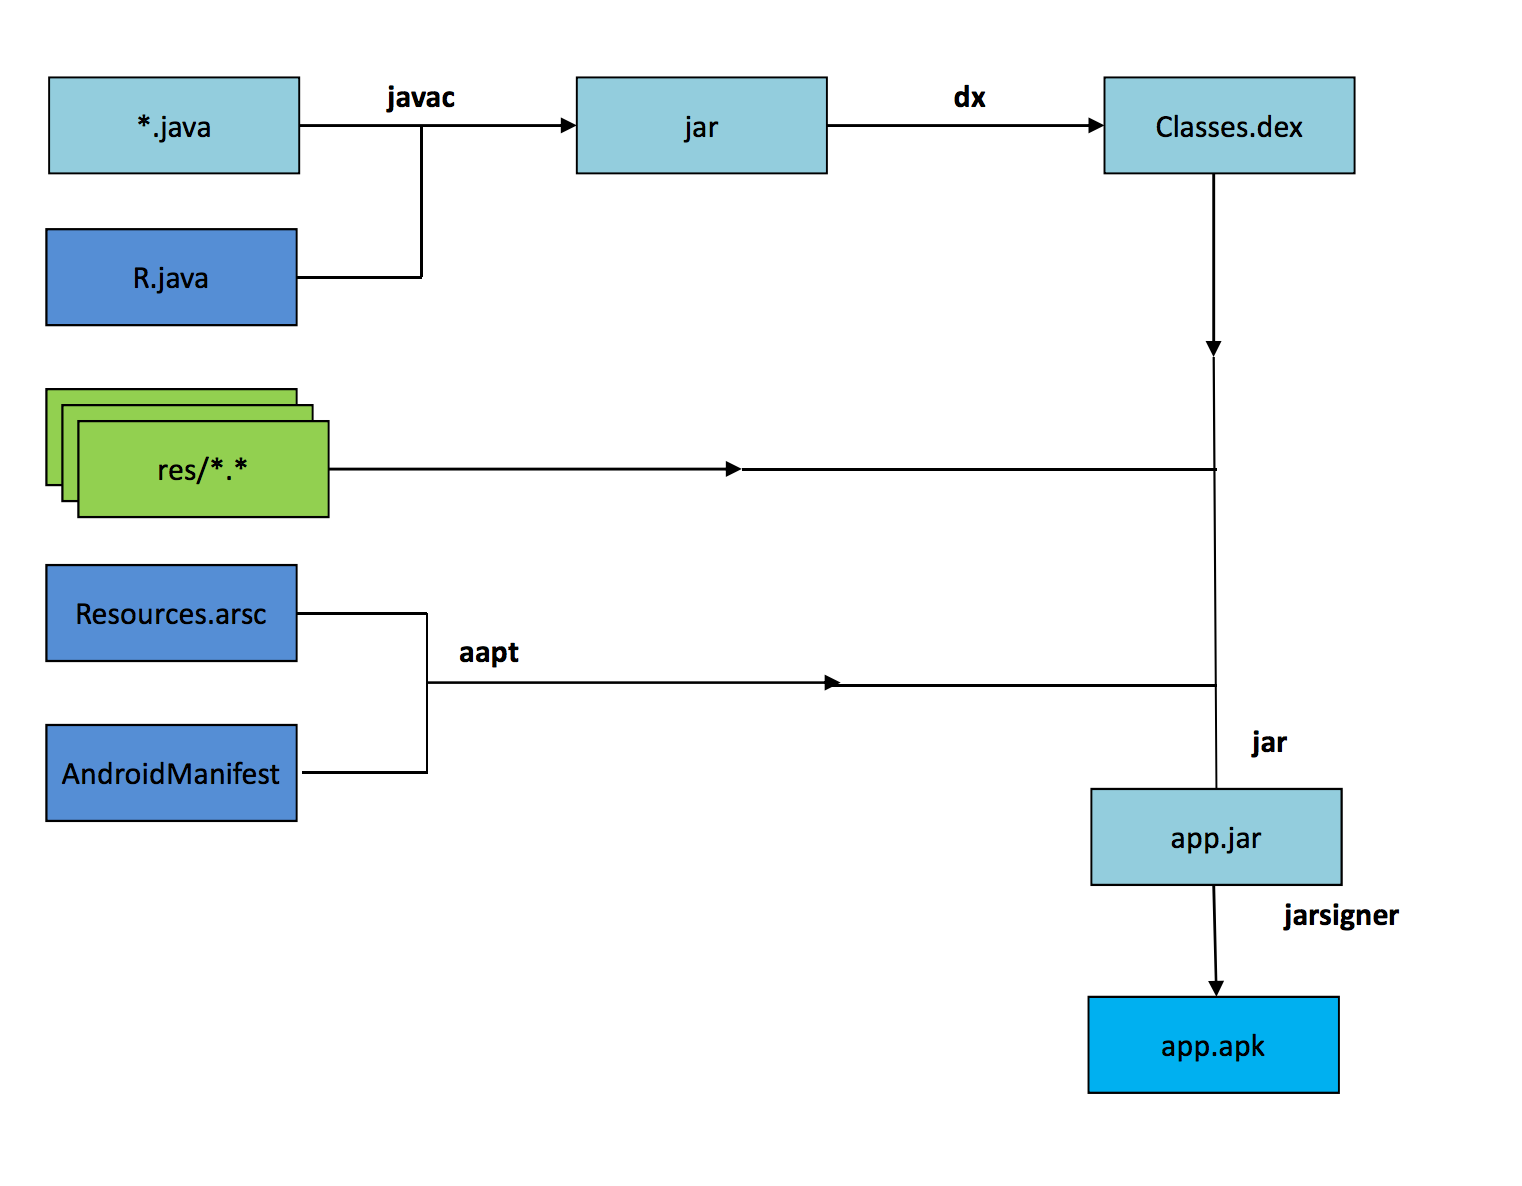
\includegraphics[width=0.8\textwidth]{data/apk.png}
    \caption{\gls{apk} build process \cite{andevconDalvikART}}
    \label{fig:apk}
\end{figure}
Since Android applications are usually written in Java, the first step is similar to the Java program build process.
The Java source code is compiled into \gls{classg} file by the Java Compiler javac.
Each .class files contains the Java bytecode of the corresponding Java class.
The structure of a \gls{classg} file can be seen in figure~\ref{fig:java}.
As an additional step in the Java compilation process a Java obfuscator can be applied (similar to section~\ref{subsection:counter-improve-obfuscation}).
In the end the .class files are packed into a \gls{jar} file.
\newline
Since Android is using the \gls{dvm}, which will be described in section~\ref{subsection:android-dalvik}, the Java bytecode has to be converted to Dalvik bytecode.
The Android \gls{sdk} includes the tool dx which is used to convert \gls{classg} files to a single classes.dex file containing all classes.
The \gls{dex} format will be described in \ref{subsection:android-dex}.
After this conversion additional obfuscation techniques can be applied \cite{dexProtector}.
\newline
In the next step the ApkBuilder combines the three main parts of the application into one archive file.
The first one is the classes.dex with the bytecode.
The second part are the resources files which are added when present.
These files are static content like images, layouts and the native code which is stored in shared object (.so) files.
The third type of files are the resources.arsc file, which contain the compiled resources, and the Android Manifest, which gives essential information like needed permissions which have to be known before running the application.
\newline
In the fourth and final step the jarsigner adds the developers signature to the package.
It does not improve security of the application itself but it makes it possible to identify the developer and by this allow actions like updates.
\newline
\newline
The final application file has the following folder structure.
It contains different subfolders like lib, res, assets and META-INF as well as the resources.arsc, classes.dex and AndroidManifest.xml files.
The lib folder contains subfolders with the compiled native code for the different processor types, like armeabi-v7a for ARM or x86 for Intel processors.
Assets, which can be accessed inside the application code using the AssetManager, are in the assets folder.
The resources are either in the res folder or, in case it is possible to compile them, stored in the resources.arsc.
The last folder is the META-INF, which is inherited from Java, stores package and extension configuration data and other \cite{metaJava}.
The classes.dex and AndroidManfiest.xml are already covered.
\cite{kovachevaMaster}\cite{ehringerDalvik}
